\documentclass[
11pt, % The default document font size, options: 10pt, 11pt, 12pt
codirector, % Uncomment to add a codirector to the title page
]{charter} 


% El títulos de la memoria, se usa en la carátula y se puede usar el cualquier lugar del documento con el comando \ttitle
\titulo{Monitoreo y control de sistemas de bombeo de agua potable de pozos profundos} 

% Nombre del posgrado, se usa en la carátula y se puede usar el cualquier lugar del documento con el comando \degreename
\posgrado{Maestría en Sistemas Embebidos} 
%\posgrado{Carrera de Especialización en Internet de las Cosas} 
%\posgrado{Carrera de Especialización en Inteligencia Artificial}
%\posgrado{Maestría en Sistemas Embebidos} 
%\posgrado{Maestría en Internet de las cosas}
% IMPORTANTE: no omitir titulaciones ni tildación en los nombres, también se recomienda escribir los nombres completos (tal cual los tienen en su documento)
% Tu nombre, se puede usar el cualquier lugar del documento con el comando \authorname
\autor{Esp. Ing. Mario Fernando Aguilar Montoya}

% El nombre del director y co-director, se puede usar el cualquier lugar del documento con el comando \supname y \cosupname y \pertesupname y \pertecosupname
\director{Mg. Ing. Mauricio Barroso Benavides}
\pertenenciaDirector{FIUBA} 
\codirector{Título y Nombre del codirector} % para que aparezca en la portada se debe descomentar la opción codirector en los parámetros de documentclass
\pertenenciaCoDirector{FIUBA}

% Nombre del cliente, quien va a aprobar los resultados del proyecto, se puede usar con el comando \clientename y \empclientename
\cliente{Ing. Carlos Alvarado}
\empresaCliente{COSAALT RL}
 
\fechaINICIO{22 de junio de 2024}		%Fecha de inicio de la cursada de GdP \fechaInicioName
\fechaFINALPlan{17 de Agosto de 2024} 	%Fecha de final de cursada de GdP
\fechaFINALTrabajo{15 de mayo de 2024}	%Fecha de defensa pública del trabajo final


\begin{document}

\maketitle
\thispagestyle{empty}
\pagebreak


\thispagestyle{empty}
{\setlength{\parskip}{0pt}
\tableofcontents{}
}
\pagebreak


\section*{Registros de cambios}
\label{sec:registro}


\begin{table}[ht]
\label{tab:registro}
\centering
\begin{tabularx}{\linewidth}{@{}|c|X|c|@{}}
\hline
\rowcolor[HTML]{C0C0C0} 
Revisión & \multicolumn{1}{c|}{\cellcolor[HTML]{C0C0C0}Detalles de los cambios realizados} & Fecha      \\ \hline
0      & Creación del documento                                 &\fechaInicioName \\ \hline
1      & Se completa hasta el punto 5 inclusive                & {2} de {agosto} de 2024 \\ \hline
%2      & Se completa hasta el punto 9 inclusive
%		  Se puede agregar algo más \newline
%		  En distintas líneas \newline
%		  Así                                                    & {día} de {mes} de 202X \\ \hline
%3      & Se completa hasta el punto 12 inclusive                & {día} de {mes} de 202X \\ \hline
%4      & Se completa el plan	                                 & {día} de {mes} de 202X \\ \hline

% Si hay más correcciones pasada la versión 4 también se deben especificar acá

\end{tabularx}
\end{table}

\pagebreak



\section*{Acta de constitución del proyecto}
\label{sec:acta}

\begin{flushright}
Buenos Aires, \fechaInicioName
\end{flushright}

\vspace{2cm}

Por medio de la presente se acuerda con el \authorname\hspace{1px} que su Trabajo Final de la \degreename\hspace{1px} se titulará ``\ttitle'' y consistirá en esencialmente en la implementación de un prototipo de un sistema de monitoreo y control de un sistema de bombeo de agua potable. El trabajo tendrá un presupuesto preliminar estimado de \textcolor{red}{600} horas y un costo estimado de \textcolor{red}{\$ XXX}, con fecha de inicio el \fechaInicioName\hspace{1px} y fecha de presentación pública el \fechaFinalName.

Se adjunta a esta acta la planificación inicial.

\vfill

% Esta parte se construye sola con la información que hayan cargado en el preámbulo del documento y no debe modificarla
\begin{table}[ht]
\centering
\begin{tabular}{ccc}
\begin{tabular}[c]{@{}c@{}}Dr. Ing. Ariel Lutenberg \\ Director posgrado FIUBA\end{tabular} & \hspace{2cm} & \begin{tabular}[c]{@{}c@{}}\clientename \\ \empclientename \end{tabular} \vspace{2.5cm} \\ 
\multicolumn{3}{c}{\begin{tabular}[c]{@{}c@{}} \supname \\ Director del Trabajo Final\end{tabular}} \vspace{2.5cm} \\
\end{tabular}
\end{table}




\section{1. Descripción técnica-conceptual del proyecto a realizar}
\label{sec:descripcion}
El objetivo principal del proyecto es la creación de un prototipo capaz de obtener mediciones de  y enviar las variables medidas a una plataforma en la nube haciendo uso de un módulo de comunicación GSM/GPRS.

En la figura \ref{fig:diagra_sistema} se puede observar el diagrama de bloques del sistema.
El proyecto permitirá al cliente disminuir el desprecio de agua que ocurre al momento de bombear agua desde los pozos profundos a lo tanques de almacenamiento y también el cliente pod 

\begin{figure}[hpb]
	\centering 
	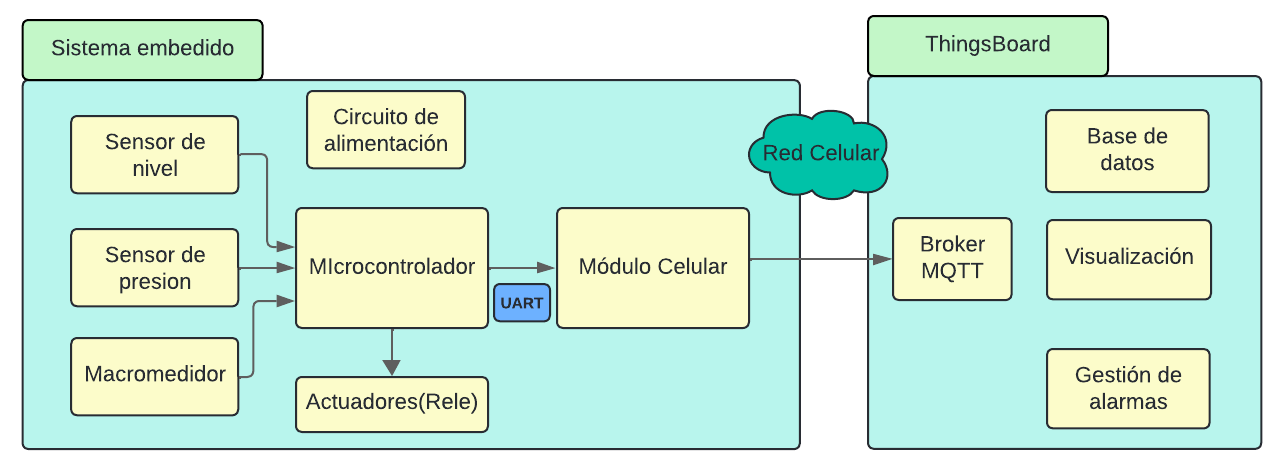
\includegraphics[width=12cm, height=6cm]{./Figuras/d_sistema.png}
	\caption{Diagrama en bloques del sistema.}
	\label{fig:diagra_sistema}
\end{figure}

\begin{consigna}{red} % El bloque "consigna" se usa para poner texto en rojo y dar una pequeña ayuda sobre cómo completar la sección. En cada entrega parcial deben eliminar los comandos begin y end del bloque consigna de las secciones que hayan completado.
El objetivo es que el lector, en una o dos páginas, exponga de qué se trata el proyecto y cuáles son sus desafíos, cuál es la motivación para realizarlo y su importancia.

Se debe introducir el contexto del proyecto, el estado del arte en la temática, describir la propuesta de valor, cuál es el problema que atiende y cuál es la solución que se propone. Se debe dar una descripción funcional de la solución que incluya un diagrama en bloques.

Puede ser útil incluir en esta sección la respuesta a alguna de estas preguntas:

\begin{itemize}
	\item ¿Cuál es el contexto del proyecto, es un emprendimiento personal, un proyecto para una empresa, es parte del programa de vinculación con empresas del posgrado?
	\item ¿Existen o aplican condiciones especiales al proyecto, financiamiento de algún programa público o privado, acuerdos de confidencialidad, acuerdos sobre la propiedad intelectual de los entregables u otros?
	\item ¿Cómo se compara la solución propuesta con el estado del arte en el campo de aplicación? ¿En qué aspectos destaca?
	\item ¿Ayuda a la explicación si se incluye un lienzo Canvas del Modelo de Negocio?
	\item ¿En qué estado del ciclo de vida está la solución que se propone?
	\item ¿Cuáles son las características del cliente (el adoptante de los entregables del proyecto) qué valora, qué necesita?
	\item ¿Por dónde pasa la innovación?
\end{itemize}

La descripción técnica-conceptual \textbf{debe incluir al menos un diagrama en bloques del sistema} y descripción funcional de la solución propuesta.

Las figuras se deben mencionar en el texto ANTES de que aparezcan con una frase como la siguiente: ``En la figura \ref{fig:diagBloques} se presenta el diagrama en bloques del sistema. Se observa que...''.  La regla es que las figuras nunca pueden ir antes de ser mencionadas en el texto, porque sino el lector no entiende por qué de pronto aparece una figura.

\begin{figure}[htpb]
\centering 
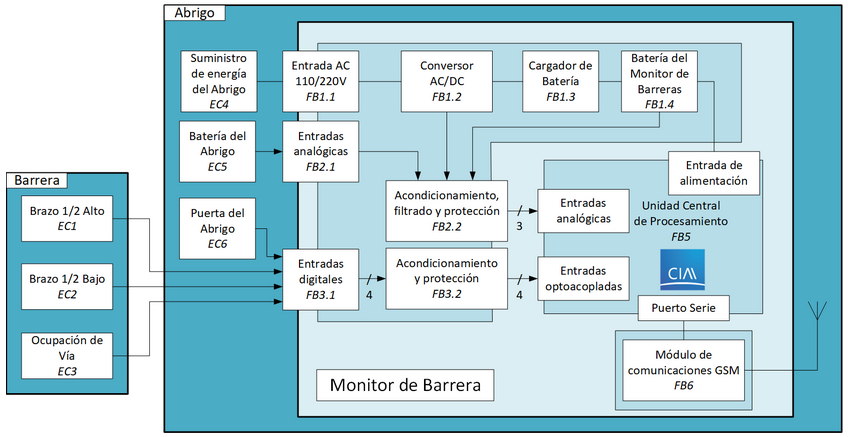
\includegraphics[width=.65\textwidth]{./Figuras/diagBloques.png}
\caption{Diagrama en bloques del sistema.}
\label{fig:diagBloques}
\end{figure}

\vspace{25px}

El tamaño del texto en TODAS las figuras debe ser adecuado \textbf{para que NO pase lo que ocurre en la figura \ref{fig:diagBloques}}, donde el lector debe esforzarse para poder leer el texto. 

Los colores usados en el diagrama deben ser adecuados, tal que ayuden a comprender mejor el diagrama. Se recomienda evitar colores primarios (como rojo, verde o cyan) y usar la gama de colores pastel.
\end{consigna}

\section{2. Identificación y análisis de los interesados}
\label{sec:interesados}

\begin{table}[ht]
%\caption{Identificación de los interesados}
%\label{tab:interesados}
\begin{tabularx}{\linewidth}{@{}|l|X|X|l|@{}}
\hline
\rowcolor[HTML]{C0C0C0} 
Rol           & Nombre y Apellido & Organización 	& Puesto 	\\ \hline
Cliente       & \clientename      &\empclientename	& -      	\\ \hline
Responsable   & \authorname       & FIUBA        	& Alumno 	\\ \hline
Orientador    & \supname	      & - 				& Director del Trabajo Final \\ \hline
Usuario final & Operarios         & -            	& -      	\\ \hline
\end{tabularx}
\end{table}

Es deseable listar a continuación las principales características de cada interesado.
\begin{itemize}
	\item Orientador: la Dra. Ing. María Gómez es experta en la temática y va a ayudar con la definición de los requerimientos y el desarrollo del firmware del embebido.
	\item Auspiciante: es riguroso y exigente con la rendición de gastos. Tener mucho cuidado con esto.
\end{itemize}



\section{3. Propósito del proyecto}
\label{sec:proposito}
El propósito del proyecto es desarrollar un sistema que sea capaz de monitorear y controlar parámetros relevantes en un sistema de bombeo de agua, con la finalidad de disminuir el consumo energético de las bombas  y el desperdicio de agua potable.

\section{4. Alcance del proyecto}
\label{sec:alcance}
El proyecto incluye:
\begin{itemize}
	\item Diseño e implementación de un prototipo y pruebas preliminares de funcionamiento.
	\item Desarrollo del firmware del microcontrolador basado en un sistema operativo de tiempo real.
	\item Configuración de la interfaz gráfica de la plataforma IoT.
\end{itemize}
El proyecto no incluye:
\begin{itemize}
	\item Diseño y fabricación del gabinete que aloja al dispositivo.
	\item Manuales de instalación y de usuario del dispositivo.
\end{itemize}

\section{5. Supuestos del proyecto}
\label{sec:supuestos}

\begin{itemize}
	\item El tiempo de fabricación de los PCBs de prueba estará dentro de lo planeado.
	\item El tiempo de importación de los módulos y componentes estarán dentro de lo planeado.
	\item El presupuesto no superará en gran medida lo estimado.
	\item No tener problemas de importación de los componentes.
	\item El tiempo de desarrollo del firmware 
	\item La situacion del pais 
	\item El tiempo de diseno del hardarew

\end{itemize}

\section{6. Requerimientos}
\label{sec:requerimientos}
\begin{enumerate}
	\item Requerimientos funcionales:
		\begin{enumerate}
			\item Requerimientos de firmware
			\begin{enumerate} 
				\item El firmware debe comunicarse con el modulo GSM/GPRS mediante protocolo serial.
				\item El firmware debe poder suscribirse y publicar en topicos utilizando el protocolo MQTT.
				\item El firmware debe estar bajo un RTOS.
				\item El firmware debe poder obtener las lecturas de los sensores.
				\item Se deben realizar los drivers para los sensores.
				\item Se debe hacer test unitarios para los drivers.
				\item Se debe hacer test de integracion.
				\item El firmware debe poder actualizarse de forma remota.
			\end{enumerate}
			\item Requerimientos de hardware
			\begin{enumerate} 
				\item El microcontrolador tiene que ser 
				\item El PCB tiene circuitos de conversion de 
				\item El PCB tiene que tener un circui
				\item El prototipo debe usar un modulo GSM/GPRS.
				\item La caja debe ser generica.
				\item Debe contar con una display.
			\end{enumerate}			
			\item Requerimientos de interfaz gráfica
			\begin{enumerate} 
				\item Debe mostrar los valores de los sensores.
				\item Debe mostrar el estado de los actuadores.
				\item Debe contar con botones para controlar la actuadores.
				\item Debe almacenar los datos.
				\item Debe poder establecer reglas y alarmas. 
			\end{enumerate}
			\item Requerimientos de documentación
			\begin{enumerate} 
				\item Se debe presentar un informe de avance del proyecto.
				\item Se debe presentar una memoria tecnica al final del proyecto.
			\end{enumerate}
		\end{enumerate}

	\item Requerimiento de testing
	\item Requerimientos de documentación:
		\begin{enumerate}
			\item Requerimiento 1.
			\item Requerimiento 2 (prioridad menor)
		\end{enumerate}

\end{enumerate}


\begin{consigna}{red}
Los requerimientos deben enumerarse y de ser posible estar agrupados por afinidad, por ejemplo:

\begin{enumerate}
	\item Requerimientos funcionales:
		\begin{enumerate}
			\item El sistema debe...
			\item Tal componente debe...
			\item El usuario debe poder...
		\end{enumerate}
	\item Requerimientos de documentación:
		\begin{enumerate}
			\item Requerimiento 1.
			\item Requerimiento 2 (prioridad menor)
		\end{enumerate}
	\item Requerimiento de testing...
	\item Requerimientos de la interfaz...
	\item Requerimientos interoperabilidad...
	\item etc...
\end{enumerate}

Leyendo los requerimientos se debe poder interpretar cómo será el proyecto y su funcionalidad.

Indicar claramente cuál es la prioridad entre los distintos requerimientos y si hay requerimientos opcionales. 

\textbf{¡¡¡No olvidarse de que los requerimientos incluyen a las regulaciones y normas vigentes!!!}

Y al escribirlos seguir las siguientes reglas:
\begin{itemize}
	\item Ser breve y conciso (nadie lee cosas largas). 
	\item Ser específico: no dejar lugar a confusiones.
	\item Expresar los requerimientos en términos que sean cuantificables y medibles.
\end{itemize}

\end{consigna}

\section{7. Historias de usuarios (\textit{Product backlog})}
\label{sec:backlog}
Se utiliza la serie de Fibonacci: 0, 1, 3, 5, 8, 13, 21, 34. . . para establecer los pesos de las historias
de usuario. Se suman los pesos de : cantidad de trabajo a realizar , complejidad del trabajo a
realizar y riesgo o incertidumbre del trabajo a realizar. Si el peso no conincide con alguno de la
serie se asigna el inmediato superior.

Tabla de pesos:
\begin{itemize}
	\item Cantidad de trabajo a realizar 
	\begin{itemize}
		\item Cantidad de trabajo a realizar 
	\end{itemize}
	\item Complejidad del trabajo a realizar
	\begin{itemize}
		\item Cantidad de trabajo a realizar 
	\end{itemize}
	\item Riesgo o incertidumbre del trabajo a realizar
	\begin{itemize}
		\item Cantidad de trabajo a realizar 
	\end{itemize}
\end{itemize}


\begin{consigna}{red}
Descripción: en esta sección se deben incluir las historias de usuarios y su ponderación (\textit{history points}). Recordar que las historias de usuarios son descripciones cortas y simples de una característica contada desde la perspectiva de la persona que desea la nueva capacidad, generalmente un usuario o cliente del sistema. La ponderación es un número entero que representa el tamaño de la historia comparada con otras historias de similar tipo.

Se debe indicar explícitamente el criterio para calcular los \textit{story points} de cada historia.

El formato propuesto es: 
\begin{enumerate}
\item ``Como [rol] quiero [tal cosa] para [tal otra cosa]."

\textit{Story points}: 8 (complejidad: 3, dificultad: 2, incertidumbre: 3)
\end{enumerate}
\end{consigna}

\section{8. Entregables principales del proyecto}
\label{sec:entregables}

\begin{itemize}
	\item Documentacion en formato pdf de los esquematicos y planos del PCB.
	\item Código fuente del firmware no editable.
	\item Prototipo funcional.
	\item documentación del proyecto.
\end{itemize}

\section{9. Desglose del trabajo en tareas}
\label{sec:wbs}

\begin{consigna}{red}
El WBS debe tener relación directa o indirecta con los requerimientos.  Son todas las actividades que se harán en el proyecto para dar cumplimiento a los requerimientos. Se recomienda mostrar el WBS mediante una lista indexada:

\begin{enumerate}
\item documentación del proyecto(suma h)
	\begin{enumerate}
	\item Planificacion del proyecto(tantas h)
	\item Especificacion de requisitos del firmware(tantas h)
	\item Definicion de las pruebas de aceptacion(tantas h)
	\end{enumerate}
\item Busqueda de material bibliografico (suma h)
	\begin{enumerate}
	\item Buscar hojas de datos de todos los componentes (tantas h)
	\item Estudiar como funciona cada uno de los componentes (tantas h)
	\item Investigar sobre dispositivos con funciones similares (tantas h)
	\end{enumerate}
\item Diseno del hardware del sistema (suma h)
	\begin{enumerate}
	\item Seleccion de componentes(tantas h)
	\item Diseno del esquematico(tantas h)
	\item Diseno de los simbolos(tantas h)
	\item Diseno del PCB(tantas h)
	\item Disenos de los componetes en 3D(tantas h)
	\end{enumerate}
\item Desarrollo del firmware(suma h)
	\begin{enumerate}
	\item Diseno de la arquitectura del firmware(tantas h)
	\item Desarrollo de los drivers del firmware(tantas h)
	\begin{enumerate}
		\item Desarrollo driver para el sensor de presion.
		\item Desarrollo del driver para el sensor de nivel.
		\item Desarrollo del driver para el macromedidor.
		\item Desarrollo del driver para el medidor de energia.
	\end{enumerate}
	\item Montar el sistema operativo.
	\item Desarrollar el modulo de la aplicación.
	\end{enumerate}
\item Configuracion de la interfaz grafica(suma h)	
    \begin{enumerate}
		\item Configuracion de los componentes en la interfaz.
		\item Configuracion del almacenamiento.
		\item Configuracion de las alarmas.
	\end{enumerate}
\item Testing(suma h)	
    \begin{enumerate}
		\item Testeo electrico del PCB.
		\item Testeo del firmware.
		\item Depuracion del firmware.
	\end{enumerate}
\item Cierre del proyecto(suma h)	
    \begin{enumerate}
		\item Informes de avance del proyecto.
		\item Elaboracion de la memoria tecnica del trabajo final.
		\item Presentacion final del proyecto.
	\end{enumerate}


\end{enumerate}

Cantidad total de horas: tantas.

\textbf{¡Importante!:} la unidad de horas es h y va separada por espacio del número. Es incorrecto escribir ``23hs".

\textbf{Se recomienda que no haya ninguna tarea que lleve más de 40 h.} De ser así se recomienda dividirla en tareas de menor duración.

\end{consigna}

\section{10. Diagrama de Activity On Node}
\label{sec:AoN}

\begin{consigna}{red}
Armar el AoN a partir del WBS definido en la etapa anterior.

Una herramienta simple para desarrollar los diagramas es el Draw.io (\url{https://app.diagrams.net/}).
\href{https://app.diagrams.net}{Draw.io}


\begin{figure}[htpb]
\centering 
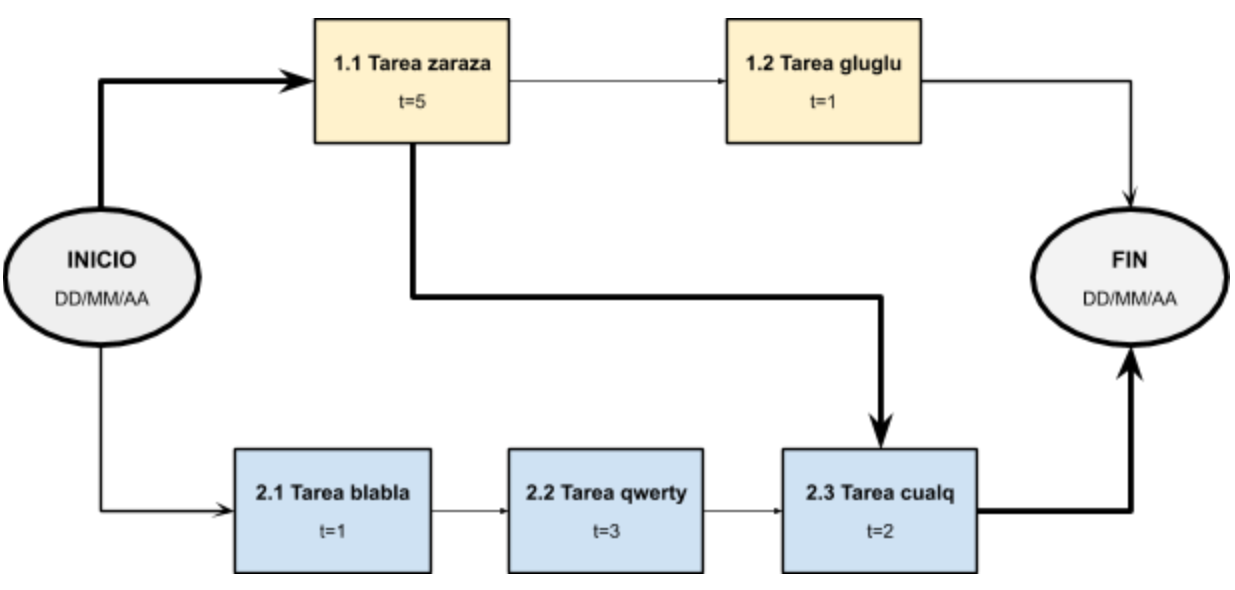
\includegraphics[width=.8\textwidth]{./Figuras/AoN.png}
\caption{Diagrama de \textit{Activity on Node}.}
\label{fig:AoN}
\end{figure}

Indicar claramente en qué unidades están expresados los tiempos.
De ser necesario indicar los caminos semi críticos y analizar sus tiempos mediante un cuadro.
Es recomendable usar colores y un cuadro indicativo describiendo qué representa cada color.

\end{consigna}

\section{11. Diagrama de Gantt}
\label{sec:gantt}

\begin{consigna}{red}
Existen muchos programas y recursos \textit{online} para hacer diagramas de Gantt, entre los cuales destacamos:

\begin{itemize}
\item Planner
\item GanttProject
\item Trello + \textit{plugins}. En el siguiente link hay un tutorial oficial: \\ \url{https://blog.trello.com/es/diagrama-de-gantt-de-un-proyecto}
\item Creately, herramienta online colaborativa. \\\url{https://creately.com/diagram/example/ieb3p3ml/LaTeX}
\item Se puede hacer en latex con el paquete \textit{pgfgantt}\\ \url{http://ctan.dcc.uchile.cl/graphics/pgf/contrib/pgfgantt/pgfgantt.pdf}
\end{itemize}

Pegar acá una captura de pantalla del diagrama de Gantt, cuidando que la letra sea suficientemente grande como para ser legible. 
Si el diagrama queda demasiado ancho, se puede pegar primero la ``tabla'' del Gantt y luego pegar la parte del diagrama de barras del diagrama de Gantt.

Configurar el software para que en la parte de la tabla muestre los códigos del EDT (WBS).\\
Configurar el software para que al lado de cada barra muestre el nombre de cada tarea.\\
Revisar que la fecha de finalización coincida con lo indicado en el Acta Constitutiva.

En la figura \ref{fig:gantt}, se muestra un ejemplo de diagrama de gantt realizado con el paquete de \textit{pgfgantt}. 
En la plantilla pueden ver el código que lo genera y usarlo de base para construir el propio.

Las fechas pueden ser calculadas utilizando alguna de las herramientas antes citadas. Sin embargo, el siguiente ejemplo
fue elaborado utilizando 
\href{https://docs.google.com/spreadsheets/d/1fBz8NhSpc4tkkhz3KjJCbh1nR_ltDkfEcZi4tZXduqs}{esta hoja de cálculo}.

Es importante destacar que el ancho del diagrama estará dado por la longitud del texto utilizado para las tareas 
(Ejemplo: tarea 1, tarea 2, etcétera) y el valor \textit{x unit}. Para mejorar la apariencia del diagrama, es necesario
ajustar este valor y, quizás, acortar los nombres de las tareas.

\begin{figure}[htpb]
  \begin{center}
    \begin{ganttchart}[
      time slot unit=day,
      time slot format=isodate,
      x unit=0.038cm,
      y unit title=0.7cm,
      y unit chart=0.6cm,
      milestone/.append style={xscale=4}
      ]{2021-03-05}{2021-12-16}
      \gantttitlecalendar*{2021-03-05}{2021-12-16}{year} \\
      \gantttitlecalendar*{2021-03-05}{2021-12-16}{month} \\
      \ganttgroup{Duración Total}{2021-03-05}{2021-12-16} \\
      %%%%%%%%%%%%%%%%%Organización
      \ganttgroup{Organización}{2021-03-05}{2021-04-16} \\
      \ganttbar{Planificación del proyecto}{2021-03-05}{2021-04-15} \\
      %%%%%%%%%%%%%%%%%Ejecución
      \ganttgroup{Ejecución}{2021-04-16}{2021-10-21} \\
      \ganttbar{Tarea 1}{2021-04-16}{2021-04-29} \\
      \ganttbar{Tarea 2}{2021-04-30}{2021-05-13} \\
      \ganttbar{Tarea 3}{2021-05-14}{2021-05-27} \\
      \ganttbar{Tarea 4}{2021-05-28}{2021-07-12} \\
      \ganttbar{Tarea 5}{2021-07-13}{2021-08-09} \\
      \ganttbar{Tarea 6}{2021-08-10}{2021-09-23} \\
      \ganttbar{Tarea 7}{2021-09-24}{2021-09-30} \\
      \ganttbar{Tarea 8}{2021-10-01}{2021-10-14} \\
      \ganttbar{Tarea 9}{2021-10-15}{2021-10-21} \\
      % %%%%%%%%%%%%%%%%%Finalización
      \ganttgroup{Finalización}{2021-10-22}{2021-12-16} \\
      \ganttbar{Memoria v1}{2021-10-22}{2021-11-04} \\
      \ganttbar{Memoria v2}{2021-11-05}{2021-11-18} \\
      \ganttbar{Memoria final}{2021-11-19}{2021-12-02} \\
      % La fecha del siguiente milestone es la fecha en que terminamos la memoria
      \ganttmilestone{Enviar memoria al director}{2021-12-02} \\
      \ganttbar{Elaborar la presentación}{2021-12-03}{2021-12-16} \\
      \ganttmilestone{Ensayo de la presentación}{2021-12-16} \\
      %%%%%%%%%%%%%%%%%%%%%%%%%%%%%%%%%%%%%%%%%%%%%%%%%%%%%%%%%%%%%%%
    \end{ganttchart}
  \end{center}
  \caption{Diagrama de gantt de ejemplo}
  \label{fig:gantt}
\end{figure}


\begin{landscape}
\begin{figure}[htpb]
\centering 
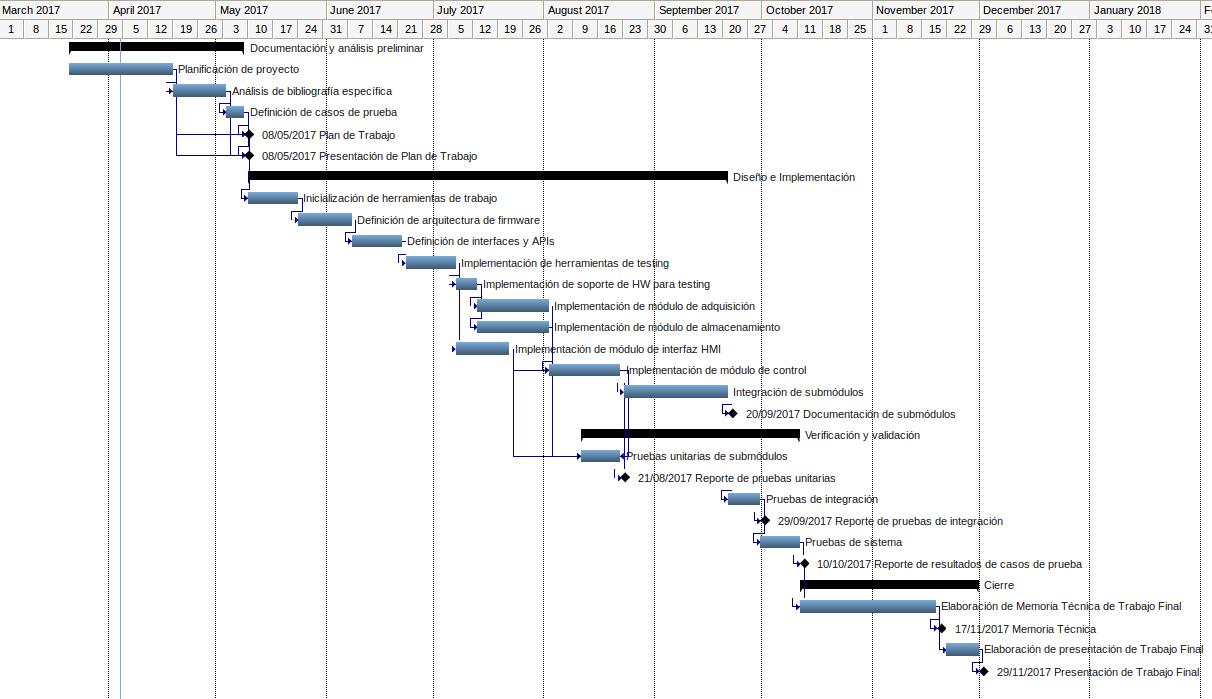
\includegraphics[height=.85\textheight]{./Figuras/Gantt-2.png}
\caption{Ejemplo de diagrama de Gantt (apaisado).} %Modificar este título acorde.
\label{fig:diagGantt}
\end{figure}

\end{landscape}

\end{consigna}


\section{12. Presupuesto detallado del proyecto}
\label{sec:presupuesto}
Los precios expresados en la siguiente tabla se encuentran en Bolivianos Bs.
\begin{consigna}{red}
Si el proyecto es complejo entonces separarlo en partes:
\begin{itemize}
	\item Un total global, indicando el subtotal acumulado por cada una de las áreas.
	\item El desglose detallado del subtotal de cada una de las áreas.
\end{itemize}

IMPORTANTE: No olvidarse de considerar los COSTOS INDIRECTOS.

Incluir la aclaración de si se emplea como moneda el peso argentino (ARS) o si se usa moneda extranjera (USD, EUR, etc). Si es en moneda extranjera se debe indicar la tasa de conversión respecto a la moneda local en una fecha dada.

\end{consigna}

\begin{table}[htpb]
\centering
\begin{tabularx}{\linewidth}{@{}|X|c|r|r|@{}}
\hline
\rowcolor[HTML]{C0C0C0} 
\multicolumn{4}{|c|}{\cellcolor[HTML]{C0C0C0}COSTOS DIRECTOS} \\ \hline
\rowcolor[HTML]{C0C0C0} 
Descripción &
  \multicolumn{1}{c|}{\cellcolor[HTML]{C0C0C0}Cantidad} &
  \multicolumn{1}{c|}{\cellcolor[HTML]{C0C0C0}Valor unitario} &
  \multicolumn{1}{c|}{\cellcolor[HTML]{C0C0C0}Valor total} \\ \hline
 Tarjeta de desarrollo&
  \multicolumn{1}{c|}{1}&
  \multicolumn{1}{c|}{150} &
  \multicolumn{1}{c|}{150} \\ \hline
 Modulo de comunicación GSM/GPRS&
  \multicolumn{1}{c|}{1} &
  \multicolumn{1}{c|}{1} &
  \multicolumn{1}{c|}{150} \\ \hline
 Componentes electronicos del PCB&
  \multicolumn{1}{c|}{1} &
  \multicolumn{1}{c|}{20} &
  \multicolumn{1}{c|}{100} \\ \hline 
 Fabricación y emsamblaje del PCB&
  \multicolumn{1}{c|}{3} &
  \multicolumn{1}{c|}{20} &
  \multicolumn{1}{c|}{60} \\ \hline 
Pantalla nextion&
  \multicolumn{1}{c|}{1} &
  \multicolumn{1}{c|}{260} &
  \multicolumn{1}{c|}{260} \\ \hline 
Caja de la tarjeta PCB&
  \multicolumn{1}{c|}{705} &
  \multicolumn{1}{c|}{50} &
  \multicolumn{1}{c|}{35250} \\ \hline
Horas de ingenieria &
  \multicolumn{1}{c|}{1} &
  \multicolumn{1}{c|}{260} &
  \multicolumn{1}{c|}{260} \\ \hline  

\multicolumn{3}{|c|}{SUBTOTAL}    360000&
  \multicolumn{1}{c|}{} \\ \hline
\rowcolor[HTML]{C0C0C0} 
\multicolumn{4}{|c|}{\cellcolor[HTML]{C0C0C0}COSTOS INDIRECTOS} \\ \hline
\rowcolor[HTML]{C0C0C0} 
Descripción &
  \multicolumn{1}{c|}{\cellcolor[HTML]{C0C0C0}Cantidad} &
  \multicolumn{1}{c|}{\cellcolor[HTML]{C0C0C0}Valor unitario} &
  \multicolumn{1}{c|}{\cellcolor[HTML]{C0C0C0}Valor total} \\ \hline
\multicolumn{1}{|l|}{30 porciento de los costos directos} &
   1&
   1&10852
   \\ \hline
\multicolumn{1}{|l|}{} &
   &
   &
   \\ \hline
\multicolumn{1}{|l|}{} &
   &
   &
   \\ \hline
\multicolumn{3}{|c|}{SUBTOTAL} &
  \multicolumn{1}{c|}{} \\ \hline
\rowcolor[HTML]{C0C0C0}
\multicolumn{3}{|c|}{TOTAL} &
   \\ \hline
\end{tabularx}%
\end{table}


\section{13. Gestión de riesgos}
\label{sec:riesgos}
a) Identificación de los riesgos (al menos cinco) y estimación de sus consecuencias:

Riesgo 1: Demora para conseguir los modulos y componentes electronicos requeridos.
\begin{itemize}
	\item Severidad (S): mientras más severo, más alto es el número (usar números del 1 al 10).\\
	Justificar el motivo por el cual se asigna determinado número de severidad (S).
	\item Probabilidad de ocurrencia (O): mientras más probable, más alto es el número (usar del 1 al 10).\\
	Justificar el motivo por el cual se asigna determinado número de (O). 
\end{itemize}  

\begin{consigna}{red}
a) Identificación de los riesgos (al menos cinco) y estimación de sus consecuencias:
 
Riesgo 1: detallar el riesgo (riesgo es algo que si ocurre altera los planes previstos de forma negativa)
\begin{itemize}
	\item Severidad (S): mientras más severo, más alto es el número (usar números del 1 al 10).\\
	Justificar el motivo por el cual se asigna determinado número de severidad (S).
	\item Probabilidad de ocurrencia (O): mientras más probable, más alto es el número (usar del 1 al 10).\\
	Justificar el motivo por el cual se asigna determinado número de (O). 
\end{itemize}   

Riesgo 2:
\begin{itemize}
	\item Severidad (S): X.\\
	Justificación...
	\item Ocurrencia (O): Y.\\
	Justificación...
\end{itemize}

Riesgo 3:
\begin{itemize}
	\item Severidad (S):  X.\\
	Justificación...
	\item Ocurrencia (O): Y.\\
	Justificación...
\end{itemize}


b) Tabla de gestión de riesgos:      (El RPN se calcula como RPN=SxO)

\begin{table}[htpb]
\centering
\begin{tabularx}{\linewidth}{@{}|X|c|c|c|c|c|c|@{}}
\hline
\rowcolor[HTML]{C0C0C0} 
Riesgo & S & O & RPN & S* & O* & RPN* \\ \hline
       &   &   &     &    &    &      \\ \hline
       &   &   &     &    &    &      \\ \hline
       &   &   &     &    &    &      \\ \hline
       &   &   &     &    &    &      \\ \hline
       &   &   &     &    &    &      \\ \hline
\end{tabularx}%
\end{table}

Criterio adoptado: 

Se tomarán medidas de mitigación en los riesgos cuyos números de RPN sean mayores a...

Nota: los valores marcados con (*) en la tabla corresponden luego de haber aplicado la mitigación.

c) Plan de mitigación de los riesgos que originalmente excedían el RPN máximo establecido:
 
Riesgo 1: plan de mitigación (si por el RPN fuera necesario elaborar un plan de mitigación).
  Nueva asignación de S y O, con su respectiva justificación:
  \begin{itemize}
	\item Severidad (S*): mientras más severo, más alto es el número (usar números del 1 al 10).
          Justificar el motivo por el cual se asigna determinado número de severidad (S).
	\item Probabilidad de ocurrencia (O*): mientras más probable, más alto es el número (usar del 1 al 10).
          Justificar el motivo por el cual se asigna determinado número de (O).
	\end{itemize}

Riesgo 2: plan de mitigación (si por el RPN fuera necesario elaborar un plan de mitigación).
 
Riesgo 3: plan de mitigación (si por el RPN fuera necesario elaborar un plan de mitigación).

\end{consigna}


\section{14. Gestión de la calidad}
\label{sec:calidad}

\begin{consigna}{red}
Elija al menos diez requerimientos que a su criterio sean los más importantes/críticos/que aportan más valor y para cada uno de ellos indique las acciones de verificación y validación que permitan asegurar su cumplimiento.

\begin{itemize} 
\item Req \#1: copiar acá el requerimiento con su correspondiente número.

\begin{itemize}
	\item Verificación para confirmar si se cumplió con lo requerido antes de mostrar el sistema al cliente. Detallar.
	\item Validación con el cliente para confirmar que está de acuerdo en que se cumplió con lo requerido. Detallar. 
\end{itemize}

\end{itemize}

Tener en cuenta que en este contexto se pueden mencionar simulaciones, cálculos, revisión de hojas de datos, consulta con expertos, mediciones, etc.  

Las acciones de verificación suelen considerar al entregable como ``caja blanca'', es decir se conoce en profundidad su funcionamiento interno.  

En cambio, las acciones de validación suelen considerar al entregable como ``caja negra'', es decir, que no se conocen los detalles de su funcionamiento interno.

\end{consigna}

\section{15. Procesos de cierre}    
\label{sec:cierre}

\begin{itemize}
	\item Pautas de trabajo que se seguirán para analizar si se respetó el Plan de Proyecto original:
	\begin{itemize}
		\item Encargado: Ing. Mario Aguilar Montoya
		\item Procedimiento: Durante el proceso de cierre se evaluara si se han cumplido los plazos
		de entrega y ejecucion de cada tarea planteada en el Plan de Proyecto.En el caso de hallar requerimientos incumplidos y/o retrasos en las
		tareas se evaluaran las causa y se propondran acciones para evitarlo en futuros
		proyectos.
	\end{itemize}
	\item Identificación de las técnicas y procedimientos útiles e inútiles que se emplearon, los problemas que surgieron y cómo se solucionaron:
	\begin{itemize}
		\item Encargado: Ing. Mario Aguilar Montoya
		\item Procedimiento: Se evaluaran los procedimientos utilizados en funcion a su utilidad
		y eficiencia para alcanzar los objetivos predefinidos.
	\end{itemize}
	\item Acto de cierre:
	\begin{itemize}
		\item Encargado: Ing. Mario Aguilar Montoya
		\item Procedimiento: Se realizara la defensa publica del trabajo final ante el jurado, posterior a esto se
		procedera a agradecer a todos los que ayudaron a realizar el proyecto, director del
		trabajo, miembros del jurado y autoridades de la CESE.
	\end{itemize}
\end{itemize}

\end{document}